\documentclass[10pt,a4paper]{article}
\usepackage[T1]{fontenc}
\usepackage[utf8]{inputenc}
\usepackage{anysize, longtable}
\usepackage{amsthm, amsfonts, amsmath, amssymb, booktabs, float}
\usepackage{sectsty, csquotes, xcolor, xspace, setspace, listings}
\usepackage{graphicx, tabularx, changepage, multirow, subcaption}
\usepackage{algorithm, algpseudocode, multicol, cuted, colortbl}
\usepackage{makecell, supertabular}
\usepackage[hidelinks,bookmarksdepth=3]{hyperref}
\usepackage[capitalise]{cleveref}
\usepackage[inline]{enumitem}
\usepackage[english]{babel}
\usepackage{microtype}
\usepackage{libertinus}
\usepackage[scale = 0.8]{plex-mono}
\usepackage[maxbibnames=99]{biblatex}
\usepackage{titlesec}
\usepackage{tikz}

\usetikzlibrary{fit, shapes.geometric, shapes.symbols, positioning, shapes.misc, calc, arrows.meta, patterns, backgrounds, decorations, decorations.markings, decorations.pathreplacing, shadows, hobby, decorations.pathmorphing}

\makeatletter

\lstdefinelanguage{Turtle}{
  morekeywords={@prefix, @base, PREFIX, BASE, a},
  morecomment=[l]{\#},
  morestring=[b]",
  sensitive=true
}

\lstdefinelanguage{SPARQL}{
  morekeywords={SELECT, CONSTRUCT, ASK, DESCRIBE, WHERE, PREFIX, BASE, FILTER, OPTIONAL, GRAPH, UNION, ORDER, BY, ASC, DESC, LIMIT, OFFSET, DISTINCT, REDUCED, BIND, AS, GROUP, HAVING},
  morecomment=[l]{\#},
  morestring=[b]",
  morestring=[b]',
  sensitive=false
}

\theoremstyle{plain}
\newtheorem{theorem}{Theorem}
\newtheorem{lemma}{Lemma}

\theoremstyle{definition}
\newtheorem{definition}{Definition}
\newtheorem{example}{Example}

\theoremstyle{remark}
\newtheorem*{note}{Note}
\newtheorem*{remark}{Remark}

\lstset{basicstyle=\setstretch{0}\small\ttfamily,breaklines=true,columns=fixed,captionpos=b,xleftmargin=0.5cm,literate={_}{\_}{1}}
\newcommand{\inlinecode}[1]{\lstinline[basicstyle=\ttfamily]$#1$}

\newlength{\offsetpage}
\newenvironment{widepage}[1][2cm]{
  \setlength{\offsetpage}{#1}
  \begin{adjustwidth}{-\offsetpage}{-\offsetpage}
  \addtolength{\linewidth}{2\offsetpage}
}{\end{adjustwidth}}

\algnewcommand{\IIf}[1]{\State \algorithmicif\ #1\ \algorithmicthen}
\algnewcommand{\IElse}[1]{\algorithmicelse\ #1}
\algnewcommand{\EndIIf}{\unskip\ \algorithmicend\ \algorithmicif}

\addbibresource{biblio.bib}

\allowdisplaybreaks
\marginsize{2.5cm}{2.5cm}{1.5cm}{1.5cm}
\setcounter{tocdepth}{2}
\setlist[itemize]{topsep=0pt, partopsep=0pt, parsep=0pt, itemsep=\parskip}
\setlist[enumerate]{topsep=0pt, partopsep=0pt, parsep=0pt, itemsep=\parskip}
\titlespacing*{\paragraph}{0pt}{0.5\baselineskip}{0.5\baselineskip}
\captionsetup[figure]{aboveskip=5pt}
\captionsetup[subfigure]{aboveskip=3pt}

\title{Semantic Integration of Geospatial Data for \\Infrastructure Vulnerability Assessment}
\author{Roland Bernard, 19598, \inlinecode{rolbernard@unibz.it}}
\date{September 2026}

\def\maketitle{
\begin{adjustwidth}{5mm}{5mm}
  \vspace{-4.5em}
  \noindent{\small\bfseries Project Report -- Data Curation 2025/2026\par}
  \vskip 0.25em
  \noindent{\LARGE\bfseries \@title\par}
  \vskip 1em
  \noindent{\large \@author\par}
  \vskip 1em
  \noindent{\small \@date\par}
  \vskip 1em
\end{adjustwidth}
}
\renewenvironment{abstract}{
  \vskip 1em
  \begin{quote}
  {\normalsize \abstractname\par}
  \small
}{
  \end{quote}
  \vskip 1em
}

\makeatother

\definecolor{unibzblue}{HTML}{0086ec}
\definecolor{unibzblue2}{HTML}{f0f8ff}

\pgfdeclarelayer{background}
\pgfdeclarelayer{foreground}
\pgfsetlayers{background,main,foreground}

\tikzset{
  flow/.style={-{Triangle[length=6, width=6]}, draw=red!70!black, very thick, shorten >= -3},
  biflow/.style={flow, {Triangle[length=6, width=6]}-{Triangle[length=6, width=6]}},
  link/.style={->, draw},
  ptr/.style={->, dashed},
  leafl/.style={-, thick},
  external/.style={inner sep=10, draw=black, fill=brown!20},
  internal/.style={inner sep=10, draw=black, fill=unibzblue!20},
  build/.style={inner sep=10, draw=black, fill=unibzblue!40},
  mixed/.style={inner sep=8.7, draw=black, path picture={
    \fill[brown!20] (path picture bounding box.south west)
      rectangle ($(path picture bounding box.north west)!.675!(path picture bounding box.north east)$);
    \fill[unibzblue!40] ($(path picture bounding box.north west)!.675!(path picture bounding box.north east)$)
      rectangle (path picture bounding box.south east);
  }},
  >=Latex, node distance=1, every node/.style={inner sep=0}
}


\begin{document}

\maketitle

\begin{abstract}
  This report details a data curation pipeline developed to assess the exposure of critical infrastructure to natural hazards, specifically landslides and avalanches, within the Bolzano region. Utilizing spatial and administrative datasets derived from the CRIMA project, the project performs extensive data profiling, including single column analysis, unique column combination, functional dependency, and inclusion dependency discovery, using the Metanome platform and YData Profiling library. The extracted metadata directly guides the design of a relational schema which is subsequently deployed in a PostGIS database. To semantically integrate this data, the project introduces an OWL 2 QL ontology representing the domain of interest. Virtual Knowledge Graph mappings are designed via the Ontop plugin for Protégé, leveraging SQL joins and spatial PostGIS functions to dynamically compute topological intersections between infrastructure elements and hazard zones. Finally, the resulting knowledge graph is exposed through a custom React-based single-page web application. By querying the Ontop SPARQL endpoint, this interface enables users to interactively analyze and identify vulnerable infrastructure assets across specific municipalities, thereby supporting evidence-based repair and maintenance planning.   
\end{abstract}


\section{Introduction} \label{into}

TODO

The idea of the project is to focus on the intersection of exposed assets and natural hazards. The aim is to identify and analyze critical infrastructure (water, electricity, and communications) that are geographically located within known hazard zones (landslides and avalanches) to assess potential vulnerabilities.

By integrating infrastructure assets with hazard inventories and administrative data, the system will be able to answer the following types of queries:
\begin{itemize}
  \item Which water-related infrastructure nodes are located within high risk landslide zones?
  \item What are the infrastructure lines that intersect with avalanche-prone areas?
  \item In a given Municipality, how many electricity lines are currently situated in a hazard zone?
  \item Which municipalities have the highest count of infrastructure elements exposed to natural hazards?
\end{itemize}

The remainder of this report is structured as follows:
\Cref{data} gives an overview of the chosen data sources. \Cref{profiling} covers the data profiling part of the project, including single column analysis in \cref{single}, \cref{ucc} covering unique column combinations, \cref{fd} containing analysis of functional dependencies, and \cref{inc} analyses inclusion dependencies. \cref{relational} describes the design and implementation of the relational database schema based on the preceding data profiling results.
\Cref{integration} covers the data integration part of the project, describing the developed ontology in \cref{ontology}, the virtual knowledge graph mappings in \cref{mappings}, and a description of the implemented application in \cref{application}.
Finally, \cref{conclusion} concludes the report with a summary of the performed tasks.



\section{Selected Data Sources} \label{data}

Following the project guidelines to integrate at least two different data sources, this project integrates five distinct datasets containing spatial and administrative information. As detailed in the guidelines, these data sources were introduced within the context of the CRIMA project. Some information about them was documented in the Teams channel of the Data Profiling module, specifically located in the folder \inlinecode{data/crima} project. Specifically, the integration will involve the following provided data sources:
\begin{itemize}
  \item \textbf{\inlinecode{bz_infrastructure_line}:} This dataset provides geometric and categorical information regarding critical infrastructure lines. It contains multi-line geometries representing physical lines alongside classifications for infrastructure types, such as power lines and water pipes. The line dataset contains 47,551 rows detailing 11 types of line infrastructure.
  \item \textbf{\inlinecode{bz_infrastructure_node}:} This dataset contains point-like critical infrastructure information. It specifies the point geometries and infrastructure types for various nodes, such as water catchments, electrical substations, and communication infrastructure. The node dataset contains 4,223 rows representing 10 types of facilities.
  \item \textbf{\inlinecode{bz_hazard_landslide}:} This source supplies information regarding known landslide risk areas. It includes polygon geometries defining the spatial extent of the hazards, alongside categorical classifications of the landslide process types and level of danger. The landslide dataset contains 23,737 records categorized into four danger levels and five specific landslide process types.
  \item \textbf{\inlinecode{bz_hazard_avalanche}:} Similar to the landslide dataset, this source provides spatial boundaries and risk evaluations for avalanche-prone areas. It includes polygon geometries, avalanche process categorizations, and danger levels. The avalanche dataset includes 13,071 records, classified like the landslide dataset by danger severity and avalanche process type.
  \item \textbf{\inlinecode{bz_admin_municipality}:} This dataset provides the administrative context for the region. It contains 116 records including polygon geometries representing municipal boundaries, names in multiple languages, and district associations. This dataset allows the system to aggregate and assign hazard risks to specific municipalities.
\end{itemize}

Originally these datasets were derived from the Bolzano Province GeoKatalog. They provide the necessary geospatial geometries and categorical data required for the domain analysis. All the datasets were provided for this project in the form of GZip compressed CSV files. All datasets include geographic information stored in the Well-Known Text format. The files contain multiple data quality issues that will be identified and resolved as part of the data profiling part of this project.




\section{Data Profiling} \label{profiling}

This section of the report discusses the data profiling part of the project. \Cref{single} covers the performed single column profiling steps, while \Cref{ucc}, \Cref{fd}, and \cref{inc} will cover respectively the application of unique column combination, functional dependency, and inclusion dependency discovery. Finally, \Cref{relational} covers the relational database schema designed for the data and how the profiling result affected design choices.

This part of the project made extensive use of the Metanome data profiling platform \cite{metanome}. Each section will detail which Metanome algorithms were used. In addition to Metanome, also the YData Profiling Python library \cite{ydataDocs} has been used for single column analysis.


\subsection{Single Column Analysis} \label{single}



\subsection{Unique Column Combination Discovery} \label{ucc}

TODO


\subsubsection{\texorpdfstring{\inlinecode{bz_infrastructure_line} and \inlinecode{bz_infrastructure_node}}{bz\_infrastructure\_line and bz\_infrastructure\_node}}

TODO

TODO


\subsubsection{\texorpdfstring{\inlinecode{bz_hazard_landslide} and \inlinecode{bz_hazard_avalanche}}{bz\_hazard\_landslide and bz\_hazard\_avalanche}}

TODO

TODO


\subsubsection{\texorpdfstring{\inlinecode{bz_admin_municipality}}{bz\_admin\_municipality}}

TODO



\subsection{Functional Dependency Discovery} \label{fd}

Metanome using the HyFD algorithm implementation has been used for the discovery of Functional dependencies in this project. This implementation is based on the hybrid approach introduced in \cite{papenbrock2016hybrid}. The results of this analysis can be used to identify parts of the tables that can possible be extracted into separate relations in the design of the relational schema for \cref{relational}.


\subsubsection{\texorpdfstring{\inlinecode{bz_infrastructure_line} and \inlinecode{bz_infrastructure_node}}{bz\_infrastructure\_line and bz\_infrastructure\_node}}

\begin{table}[ht!]
  \begin{widepage}
    \centering
    \begin{tabular}{|l|r|}
    \hline
      Determinant & Dependents \\ \hline \hline
      \{\} & \inlinecode{codealt}, \inlinecode{blp} \\ \hline
      \{\inlinecode{ogc_fid}\} & \ast \\ \hline
      \{\inlinecode{gml_id}\} & \ast \\ \hline
      \{\inlinecode{objectid}\} & \ast \\ \hline
      \{\inlinecode{geom}\} & \inlinecode{istat_code}, \inlinecode{nda_link_de}, \inlinecode{nda_link_it} \inlinecode{gem_text_d}, \inlinecode{gem_text_i}, \inlinecode{nda_text_de} \\ \hline
      \{\inlinecode{shape_len}\} & \inlinecode{nda_text_de}, \inlinecode{nda_text_it} \\ \hline
      \{\inlinecode{istat_code}\} & \inlinecode{nda_link_de}, \inlinecode{nda_link_it}, \inlinecode{gem_text_d}, \inlinecode{gem_text_i}, \inlinecode{nda_text_de}, \inlinecode{csv.nda_text_it} \\ \hline
      \{\inlinecode{nda_link_de}\} & \inlinecode{istat_code}, \inlinecode{nda_link_it}, \inlinecode{gem_text_d}, \inlinecode{gem_text_i}, \inlinecode{nda_text_de}, \inlinecode{nda_text_it} \\ \hline
      \{\inlinecode{csv.nda_link_it}\} & \inlinecode{istat_code}, \inlinecode{nda_link_de}, \inlinecode{gem_text_d}, \inlinecode{gem_text_i}, \inlinecode{nda_text_de}, \inlinecode{nda_text_it} \\ \hline
      \{\inlinecode{gem_text_d}\} & \inlinecode{istat_code}, \inlinecode{nda_link_de}, \inlinecode{nda_link_it}, \inlinecode{gem_text_i}, \inlinecode{nda_text_de}, \inlinecode{nda_text_it} \\ \hline
      \{\inlinecode{gem_text_i}\} & \inlinecode{istat_code}, \inlinecode{nda_link_de}, \inlinecode{nda_link_it}, \inlinecode{gem_text_d}, \inlinecode{nda_text_de}, \inlinecode{nda_text_it} \\ \hline
      \{\inlinecode{code}\} & \inlinecode{bez_i}, \inlinecode{bez_d} \\ \hline
      \{\inlinecode{bez_i}\} & \inlinecode{code}, \inlinecode{bez_d} \\ \hline
      \{\inlinecode{bez_d}\} & \inlinecode{code}, \inlinecode{bez_i} \\ \hline
      \{\inlinecode{nda_text_de}\} & \inlinecode{nda_text_it} \\ \hline
      \{\inlinecode{nda_text_it}\} & \inlinecode{nda_text_de} \\ \hline
    \end{tabular}
  \end{widepage}
  \caption{Functional dependencies discovered in \inlinecode{bz_infrastructure_line} table using the Metanome HyFD algorithm. Multiple columns in the dependents means that all of them are functionally dependent on the determinant. Further, unique column combinations have been marked with \ast.}
  \label{tab:bz_infrastructure_line_fd}
\end{table}

TODO

\begin{table}[ht!]
  \begin{widepage}
    \centering
    \begin{tabular}{|l|r|}
    \hline
      Determinant & Dependents \\ \hline \hline
      \{\} & \inlinecode{codealt} \\ \hline
      \{\} & \inlinecode{nda_text_de} \\ \hline
      \{\} & \inlinecode{nda_text_it} \\ \hline
      \{\} & \inlinecode{blp} \\ \hline
      \{\inlinecode{ogc_fid}\} & \ast \\ \hline
      \{\inlinecode{gml_id}\} & \ast \\ \hline
      \{\inlinecode{objectid}\} & \ast \\ \hline
      \{\inlinecode{geom}\} & \inlinecode{istat_code}, \inlinecode{nda_link_de}, \inlinecode{nda_link_it}, \inlinecode{gem_text_d}, \inlinecode{gem_text_i}, \inlinecode{code}, \inlinecode{bez_i}, \inlinecode{bez_d} \\ \hline
      \{\inlinecode{istat_code}\} & \inlinecode{nda_link_de}, \inlinecode{nda_link_it}, \inlinecode{gem_text_d}, \inlinecode{gem_text_i} \\ \hline
      \{\inlinecode{nda_link_de}\} & \inlinecode{istat_code}, \inlinecode{gem_text_d}, \inlinecode{gem_text_i} \\ \hline
      \{\inlinecode{nda_link_it}\} & \inlinecode{istat_code}, \inlinecode{nda_link_de}, \inlinecode{gem_text_d}, \inlinecode{gem_text_i} \\ \hline
      \{\inlinecode{gem_text_d}\} & \inlinecode{istat_code}, \inlinecode{nda_link_de}, \inlinecode{nda_link_it}, \inlinecode{gem_text_i} \\ \hline
      \{\inlinecode{gem_text_i}\} & \inlinecode{istat_code}, \inlinecode{nda_link_de}, \inlinecode{nda_link_it}, \inlinecode{gem_text_d} \\ \hline
      \{\inlinecode{code}\} & \inlinecode{bez_i}, \inlinecode{bez_d} \\ \hline
      \{\inlinecode{bez_i}\} & \inlinecode{code}, \inlinecode{bez_d} \\ \hline
      \{\inlinecode{bez_d}\} & \inlinecode{code}, \inlinecode{bez_i} \\ \hline
    \end{tabular}
  \end{widepage}
  \caption{Functional dependencies discovered in \inlinecode{bz_infrastructure_node} table using the Metanome HyFD algorithm. Multiple columns in the dependents means that all of them are functionally dependent on the determinant. Unique column combinations have been marked with \ast as dependents for brevity.}
  \label{tab:bz_infrastructure_node_fd}
\end{table}

TODO


\subsubsection{\texorpdfstring{\inlinecode{bz_hazard_landslide} and \inlinecode{bz_hazard_avalanche}}{bz\_hazard\_landslide and bz\_hazard\_avalanche}}

TODO

TODO


\subsubsection{\texorpdfstring{\inlinecode{bz_admin_municipality}}{bz\_admin\_municipality}}

TODO




\subsection{Inclusion Dependency Discovery} \label{inc}



\subsection{Relational Database Schema} \label{relational}

TODO




\section{Data Integration} \label{integration}


\subsection{Ontology} \label{ontology}

An OWL 2 QL ontology that contains relevant classes and properties has been developed as part of the project. \Cref{fig:ontology} depicts the ontology using the graphical notation introduced in the course.

\begin{figure*}[ht!]
  \centering
  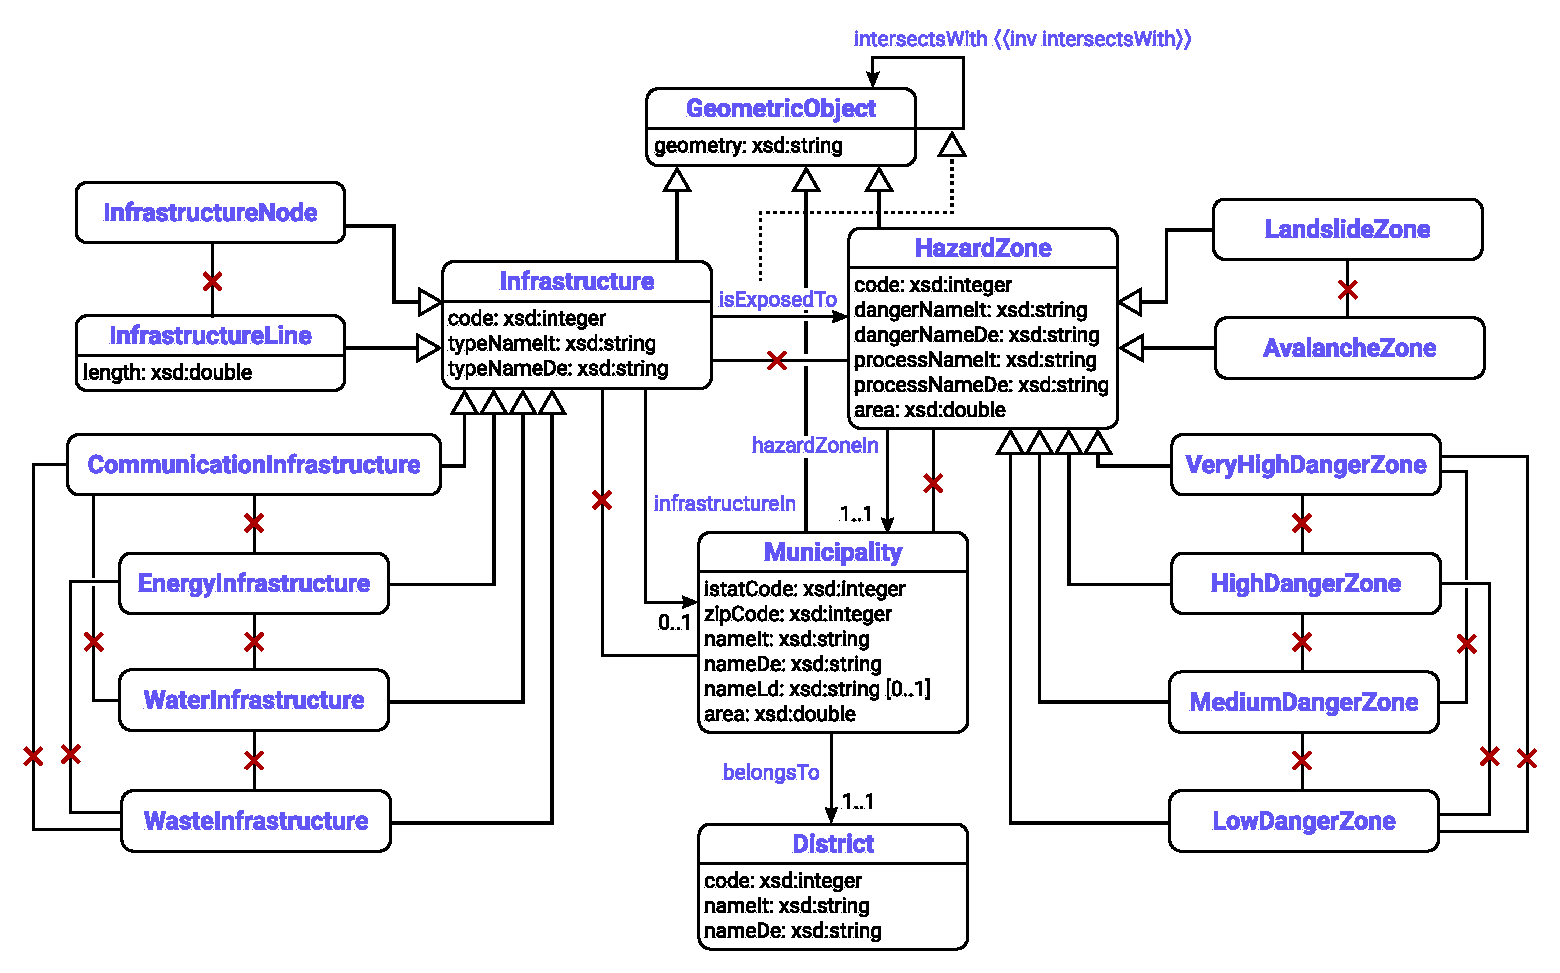
\includegraphics[width=\linewidth]{figures/ontology.pdf}
  \caption{The OWL 2 QL ontology that has been developed for the project. The diagram uses the graphical notation introduced in the course.}
  \label{fig:ontology}
\end{figure*}




\subsection{Virtual Knowledge Graph Mappings} \label{mappings}

The virtual knowledge graph mappings from the relational schema defined in \cref{relational} to the ontology covered in \cref{ontology} has been performed using the Ontop plugin for Protégé \cite{calvanese2016ontop}. This section lists and describes a representative subset of the developed mappings.

\subsubsection{IRI Generation and Base Instantiation}

The Ontop virtual knowledge graph fundamentally relies on generating unique, persistent Internationalized Resource Identifiers (IRIs) for every entity in the relational database. This is achieved using URI templates defined in the target clauses of the mappings, which bind primary keys from the relational schema to the namespace of the ontology. The templates \inlinecode{:district/\{code\}}, \inlinecode{:municipality/\{istat_code\}}, \inlinecode{:infrastructure-line/\{code\}}, \inlinecode{:infrastructure-node/\{code\}}, \inlinecode{:hazard-landslide/\{code\}}, and \inlinecode{:hazard-avalanche/\{code\}} are used in the developer mappings for the districts, municipalities, infrastructure lines, infrastructure node, landslide zones, and avalanche zones respectively. This guarantee that each physical or administrative object is represented as a distinct web resource. Note that both the infrastructure line and nodes as well as hazard zones are all collected into the different IRI temples. This is not strictly necessary, because as has been discovered during data profiling, the primary key space for the two tables is disjoint. However, making them use different IRI templates make the intention clearer and could possibly be used for some optimization. By consistently reusing these templates across all the mapping declarations, the virtual knowledge graph seamlessly merges data from disparate relational queries into a unified graph, allowing properties and classifications to be appended to the same entity incrementally.


\subsubsection{Simple Mappings}

MAP-DISTRICT

\begin{figure}[h!]
  \centering
  \begin{minipage}[t]{0.48\textwidth}
    \centering
    \textit{Source: SQL Query}
\begin{lstlisting}[language=SQL]
SELECT code, name_it, name_de
FROM District
\end{lstlisting}
  \end{minipage}
  \hfill
  \begin{minipage}[t]{0.48\textwidth}
    \centering
    \textit{Target: Triples Template}
\begin{lstlisting}[language=Turtle]
:district/{code} a :District ;
  :districtCode {code}^^xsd:integer ;
  :districtNameIt {name_it}^^xsd:string ;
  :districtNameDe {name_de}^^xsd:string .
\end{lstlisting}
  \end{minipage}
\end{figure}

MAP-MUNICIPALITY
MAP-INFRASTRUCTURE-LINE
MAP-INFRASTRUCTURE-NODE
MAP-HAZARD-LANDSLIDE
MAP-HAZARD-AVALANCHE

\subsubsection{Properties Requiring Relational Joins}

MAP-INFRASTRUCTURE-LINE-TYPE
MAP-INFRASTRUCTURE-NODE-TYPE
MAP-HAZARD-LANDSLIDE-DANGER
MAP-HAZARD-LANDSLIDE-PROCESS
MAP-HAZARD-AVALANCHE-DANGER
MAP-HAZARD-AVALANCHE-PROCESS

\subsubsection{Semantic Sub-classification}

MAP-INFRASTRUCTURE-LINE-ENERGY
MAP-INFRASTRUCTURE-LINE-WATER
MAP-INFRASTRUCTURE-LINE-WASTE
MAP-INFRASTRUCTURE-NODE-COMMUNICATION
MAP-INFRASTRUCTURE-NODE-ENERGY
MAP-INFRASTRUCTURE-NODE-WATER
MAP-INFRASTRUCTURE-NODE-WASTE
MAP-HAZARD-LANDSLIDE-VERYHIGH
MAP-HAZARD-LANDSLIDE-HIGH
MAP-HAZARD-LANDSLIDE-MEDIUM
MAP-HAZARD-LANDSLIDE-LOW
MAP-HAZARD-AVALANCHE-VERYHIGH
MAP-HAZARD-AVALANCHE-HIGH
MAP-HAZARD-AVALANCHE-MEDIUM
MAP-HAZARD-AVALANCHE-LOW

\subsubsection{Spatial Object Properties}

MAP-ISEXPOSEDTO-LINE-LANDSLIDE
MAP-ISEXPOSEDTO-LINE-AVALANCHE
MAP-ISEXPOSEDTO-NODE-LANDSLIDE
MAP-ISEXPOSEDTO-NODE-AVALANCHE
MAP-INTERSECTSWITH-LINE-MUNICIPALITY
MAP-INTERSECTSWITH-NODE-MUNICIPALITY
MAP-INTERSECTSWITH-LANDSLIDE-MUNICIPALITY
MAP-INTERSECTSWITH-AVALANCHE-MUNICIPALITY
MAP-INTERSECTSWITH-LINE-NODE
MAP-INTERSECTSWITH-LANDSLIDE-AVALANCHE
MAP-INTERSECTSWITH-LINE-LINE
MAP-INTERSECTSWITH-NODE-NODE
MAP-INTERSECTSWITH-LANDSLIDE-LANDSLIDE
MAP-INTERSECTSWITH-AVALANCHE-AVALANCHE
MAP-INTERSECTSWITH-MUNICIPALITY-MUNICIPALITY




\subsection{Application} \label{application}

The application for this project has been implemented as a custom single-page web application using Vite \cite{viteDocs}, React \cite{reactDocs} and React Router \cite{reactRouterDocs}. It offers an interactive map and results table which dynamically update based on a number of different configurations options provided to the user. To obtain the results of the queries, the application connects to the running Ontop system via its SPARQL \cite{hogan2020sparql} endpoint.

\begin{figure}[ht!]
    \centering
    \hfill
    \begin{subfigure}[t]{0.48\linewidth}
        \centering
        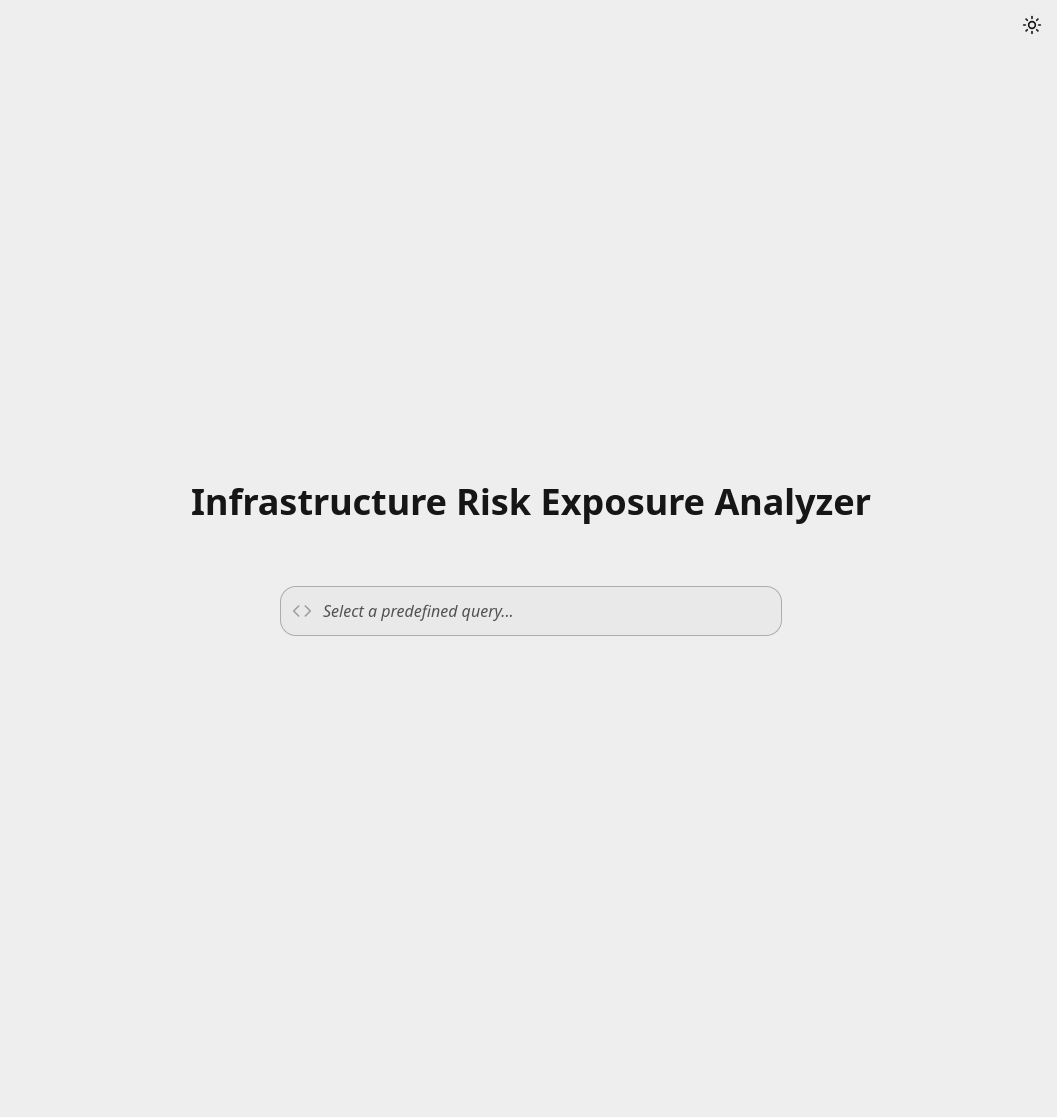
\includegraphics[width=\linewidth]{figures/home.png}
        \caption{Example screenshot of the landing page of the application. In the very center of the page there is a search bar with which the user can select one of the predefined configurations.}
        \label{fig:home}
    \end{subfigure}
    \hfill
    \begin{subfigure}[t]{0.48\linewidth}
        \centering
        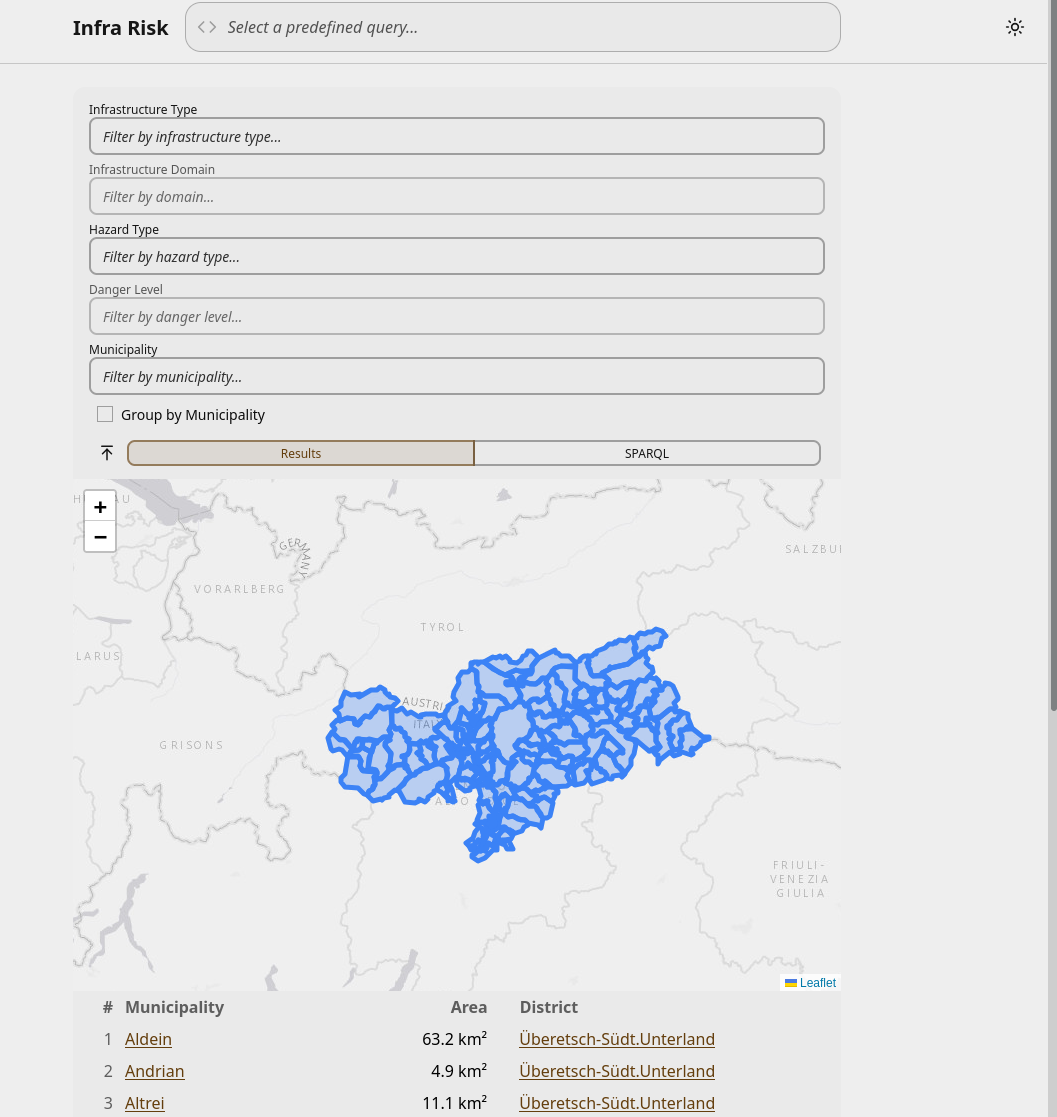
\includegraphics[width=\linewidth]{figures/municipalities.png}
        \caption{Example screenshot of the application returning the result for a simple query listing all municipalities in the knowledge graph. Below the header, which contains the search bar for selecting other predefined queries, the application lists a number of configuration options to customize the query.}
        \label{fig:municipalities}
    \end{subfigure}
    \hfill
    \caption{Example screenshot extracted from the application showing how it can be configured manually or using predefined queries.}
    \label{fig:example1}
\end{figure}

The main SPARQL query used for with the Ontop endpoint is generated dynamically based on the configurations made by the user. A small number of queries has been predefined, each serving as the answer to a concrete question related to the chosen domain. Note that these are simply configuring the exact same options that are also made available directly to the user, and do not include any special cases. \Cref{fig:home} shows how these can be selected from the home screen of the application. When inside any other screen, the predefined queries can still be accessed easily with the search bar located in the application header.

However, it is not necessary to restrict oneself to the predefined queries. \Cref{fig:municipalities} show the set of available configurable values. The first option field allows selecting the type of infrastructure to consider, lines or nodes. The second relates to the infrastructure domain, possibly filtering based on water, energy, waste, communication, or electricity related assets. Similarly to the infrastructure, also the hazards have a configurable field for whether to include avalanches, landslides, both, or neither. For the hazard zones a fourth configuration field allows selecting the danger levels to consider in the queries. Finally, it is possible to configure only a subset of municipalities to analyze, and optionally to aggregate the result by municipality. The latter is useful for answering questions about the number of vulnerable infrastructure assert per municipality. Taken together these configuration options are sufficient to implement all four example application questions that have been formulated in \cref{into} of the report. For example, by not selecting any hazard type, the query is transformed into one that returns all infrastructure assets regardless of exposure. Similarly by not selecting any infrastructure type, the query is adapted to one that instead searches for hazard zones instead of infrastructure types. Removing all types for both infrastructure and hazard results in a query simply retrieving all municipalities, corresponding to what is shown in \cref{fig:municipalities}. As soon as the user modifies some options, a new query is generated from it and executed against the Ontop endpoint to update the user interface as soon as the results have been received. A loading animation is shown while the application awaits the reception of the results to the latest query.

\begin{figure}[ht!]
    \centering
    \hfill
    \begin{subfigure}[t]{0.48\linewidth}
        \centering
        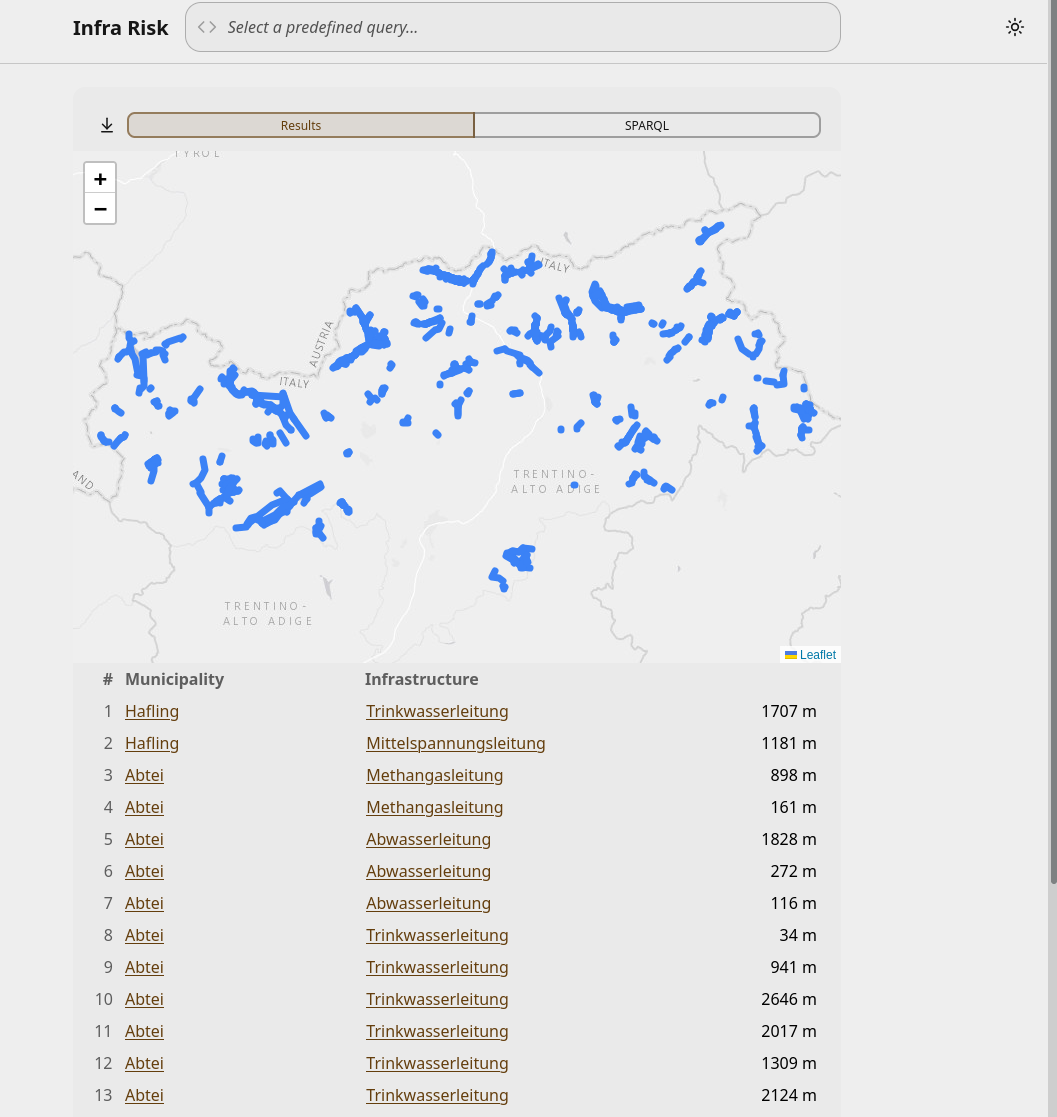
\includegraphics[width=\linewidth]{figures/avalanche.png}
        \caption{Screenshot of the application showing the results for a more complicated query involving the discovery of vulnerable infrastructure lines. The results of the currently configured query are displayed both as a map and as a table.}
        \label{fig:avalanche}
    \end{subfigure}
    \hfill
    \begin{subfigure}[t]{0.48\linewidth}
        \centering
        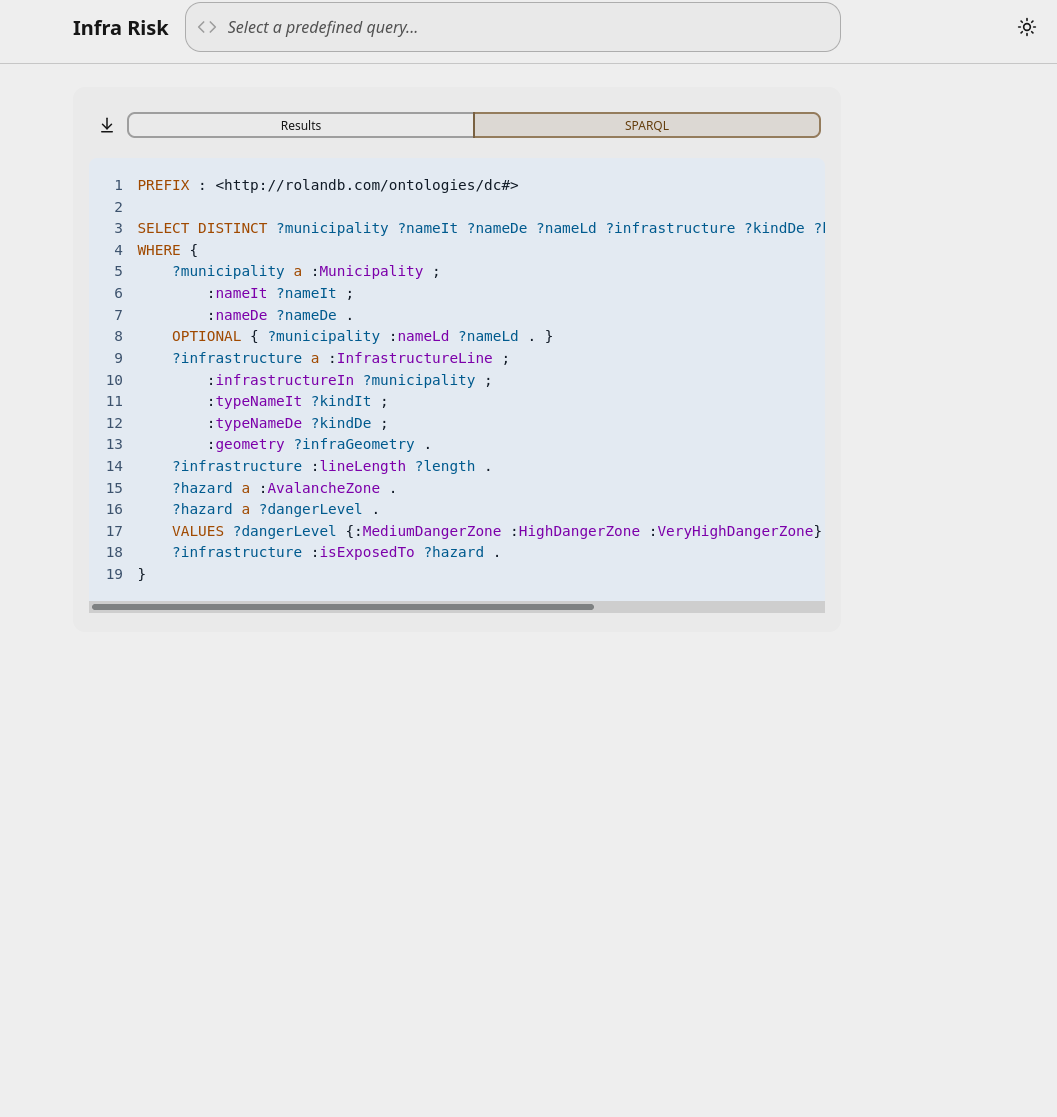
\includegraphics[width=\linewidth]{figures/sparql.png}
        \caption{Screenshot of the application showing the ability to display the SPARQL query that is being used to retrieve the results given the current configuration of the application.}
        \label{fig:sparql}
    \end{subfigure}
    \hfill
    \caption{Example screenshot extracted from the application showing how results are displayed.}
    \label{fig:example2}
\end{figure}



\begin{figure}[ht!]
    \centering
    \hfill
    \begin{subfigure}[t]{0.48\linewidth}
        \centering
        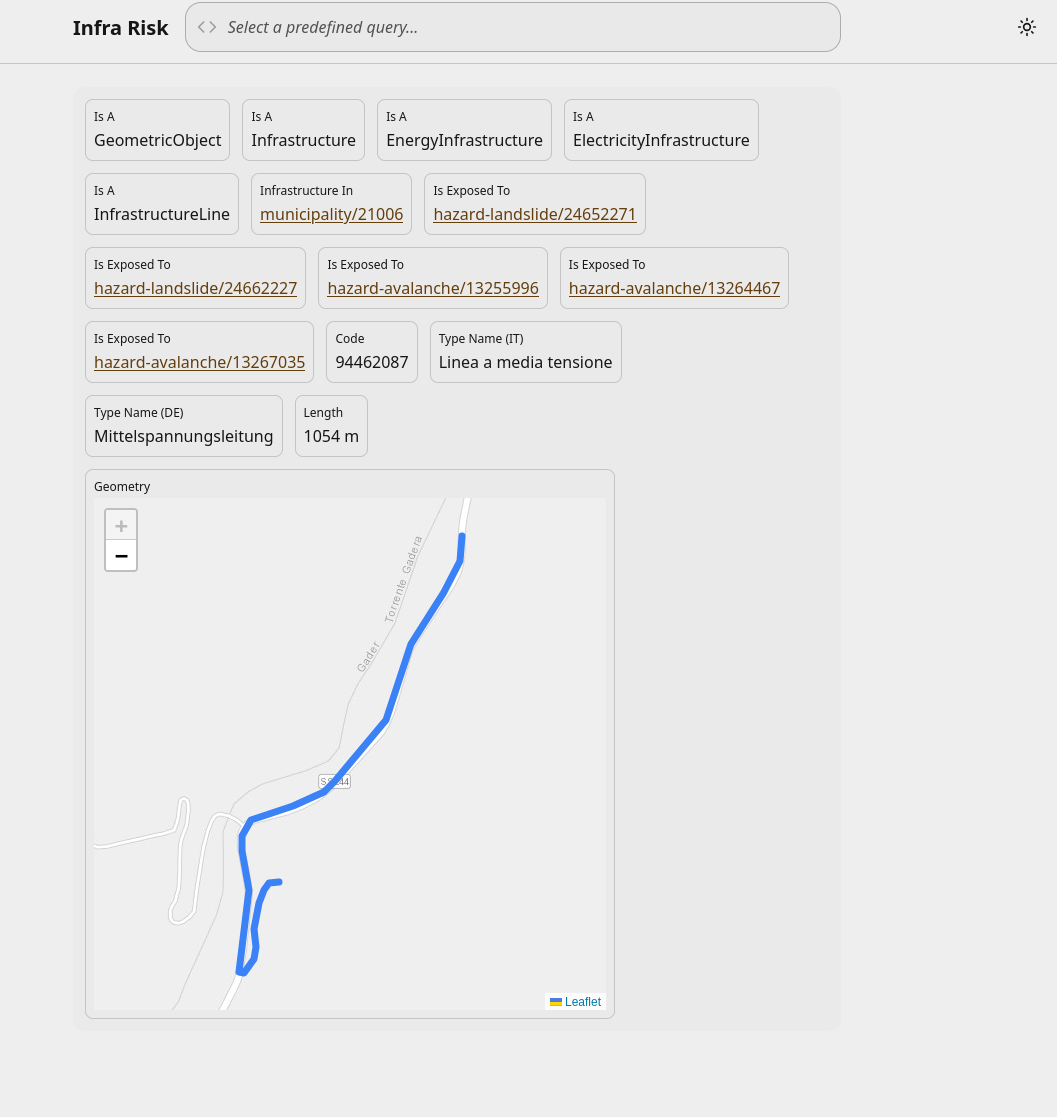
\includegraphics[width=\linewidth]{figures/infrastructure.png}
        \caption{Application screenshot that shows details regarding one specific infrastructure line.}
        \label{fig:infrastructure}
    \end{subfigure}
    \hfill
    \begin{subfigure}[t]{0.48\linewidth}
        \centering
        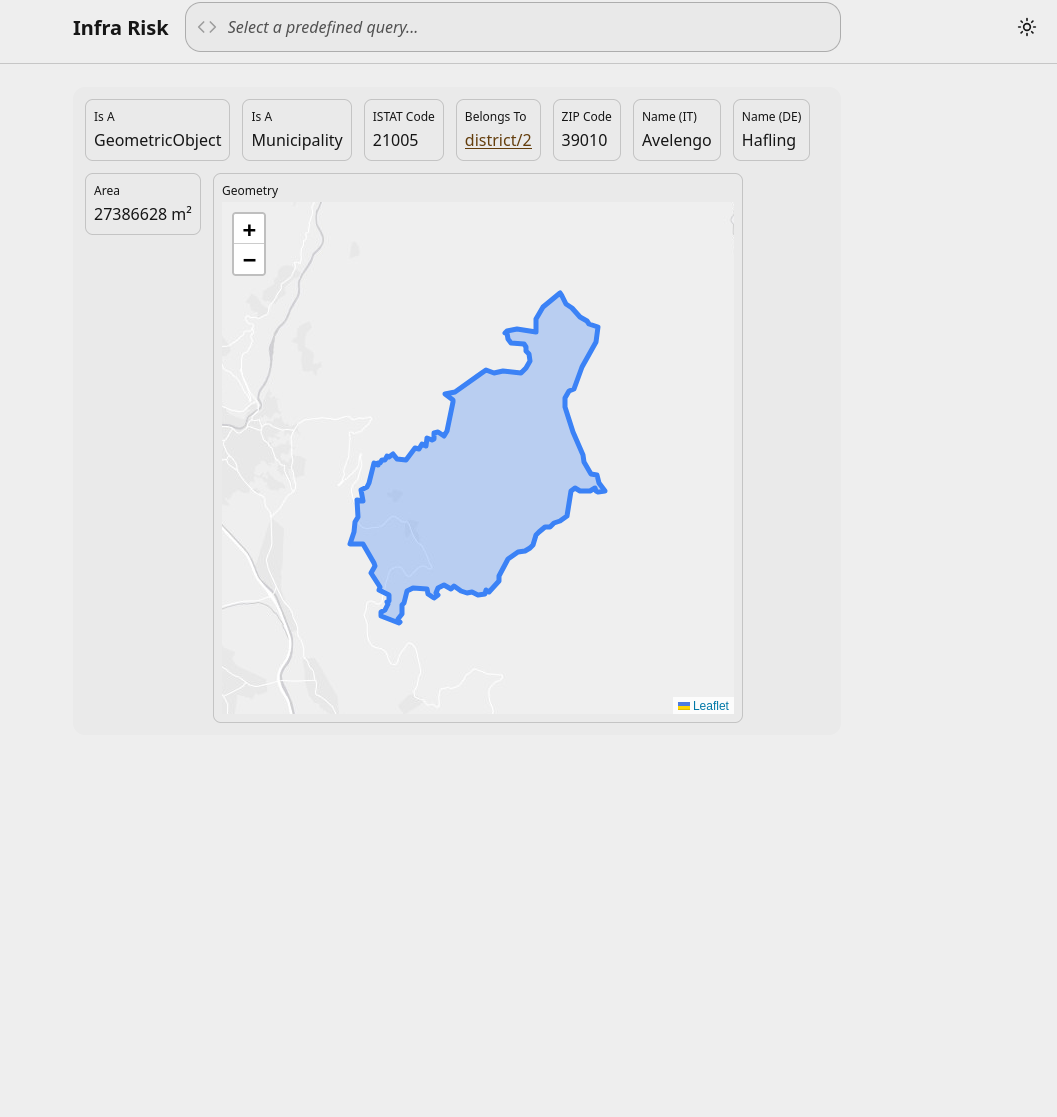
\includegraphics[width=\linewidth]{figures/municipality.png}
        \caption{Screenshot of the application showing the details for a single municipality.}
        \label{fig:municipality}
    \end{subfigure}
    \hfill
    \caption{Example screenshot extracted from the application showing the dedicated pages related to individual entities.}
    \label{fig:example3}
\end{figure}




\section{Conclusion} \label{conclusion}

TODO


\printbibliography

\end{document}
